% id: 0521
% book: RPM 중3-2 수학 · 04 원주각
% section: 실력 UP
% figure: crop:fig-0521.png
% answer: ⑤
% answer_source: 답지
% variant_level: 0 (원본 전사)
% 이 파일은 build.mjs 가 items.json 에서 만든다. 고칠 때는 items.json 을 고친다.
\noindent\begin{minipage}[t]{0.58\linewidth}\vspace{0pt}\raggedright 오른쪽 그림에서 직선~$\pt{AB}$는 두 원~$\pt{O}$, $\pt{O'}$의 접선이고 두 점~$\pt{A}$, $\pt{B}$는 접점이다. 두 점~$\pt{P}$, $\pt{Q}$는 두 원의 교점이고 $\angle\pt{PAQ}=40^\circ$, $\angle\pt{PBQ}=52^\circ$일 때, $\angle\pt{APB}$의 크기는?\end{minipage}\hfill\begin{minipage}[t]{0.4\linewidth}\vspace{0pt}\centering \setlength{\dmfigw}{96.1pt}\ifdim\dmfigw>\linewidth\setlength{\dmfigw}{\linewidth}\fi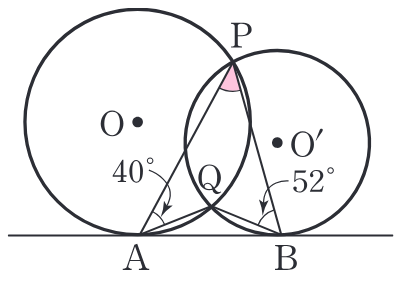
\includegraphics[width=\dmfigw]{figures/fig-0521.png}\end{minipage}\par
\dmchoicesauto{}{$40^\circ$}{$41^\circ$}{$42^\circ$}{$43^\circ$}{$44^\circ$}
